\documentclass{article}
\textheight = 25cm
% largo texto impreso
\textwidth = 18cm % ancho texto impreso
\topmargin = -2cm % margen superior 3-2=1cm
\oddsidemargin = -2cm
% margen izquierdo 4.5-2=2.5cm
% Sangría=0mm
\parindent = 0mm
\usepackage{graphicx}
\usepackage[T1]{fontenc} % fuentes adecuadas para salida % acentos,etc., desde el teclado
\usepackage{amsmath,amssymb,amsfonts,latexsym}
\usepackage{graphicx}
\usepackage[shortlabels]{enumitem}
\usepackage{esvect}
\usepackage{mathtools}
\usepackage{graphicx}
\usepackage[a4paper,margin=2cm,noheadfoot]{geometry}
\usepackage{float}
\usepackage{xspace,color}
\usepackage{url}
\usepackage{listings}



\lstset{commentstyle=\color{red},keywordstyle=\color{black},
showstringspaces=false}
\lstnewenvironment{rc}[1][]{\lstset{language=R}}{}
\newcommand{\ri}[1]{\lstinline{#1}}  %% Short for 'R inline'

\lstset{language=R} 
\begin{document}

  \parbox{3.3cm}{
\includegraphics[width=3cm]{usblogo.eps}}\parbox{8cm}{Universidad
   Sim\'on Bol\'ivar\\
   Departamento de C\'omputo Cientifico y Estadistica
   \hspace{1cm}CO5316 An\'alisis de Datos\\
   Informe an\'alisis exploratorio}\parbox{17cm}{ \hspace{1cm}Alimi Garmendia 14-10392\\
  \hspace*{1cm}Rafael \\
  \hspace*{1cm}Orlando \\
   \hspace*{1cm}Enero 2020}
   \vspace{1cm}

    En este informe nos enfocaremos en los alumnos de la raza etnica C, por lo cual comenzaremos an\'alizando
    su representaci\'on en el sal\'on y compararemos su desempe\~no en las materias.
    

    \begin{figure}[h]
        \includegraphics[scale = 0.8]{Output/Plots/RepresentacionPorRaza.eps}
        \caption{Representaci\'on del sal\'on por raza \'etnica}
        \label{fig:minipage1}
    \end{figure}


De la figura 1 podemos ver que los alumnos de raza C representan el 31.9\% del sal\'on. Debido a esto, al ser mayor\'ia,
su desempe\~no afecta sustancialmente al desempe\~no global del sal\'on.



Podemos ver como se representa esto al ver los est\'adisticos del grupo:
\begin{rc}

    math.score    reading.score   writing.score   
Min.   : 0.00   Min.   : 17.0   Min.   : 10.00  
1st Qu.:55.00   1st Qu.: 60.0   1st Qu.: 57.00  
Median :65.00   Median : 71.0   Median : 68.00  
Mean   :64.46   Mean   : 69.1   Mean   : 67.83  
3rd Qu.:74.00   3rd Qu.: 78.5   3rd Qu.: 79.00  
Max.   :98.00   Max.   :100.0   Max.   :100.00
\end{rc}
\begin{figure}[H]
    \centering
    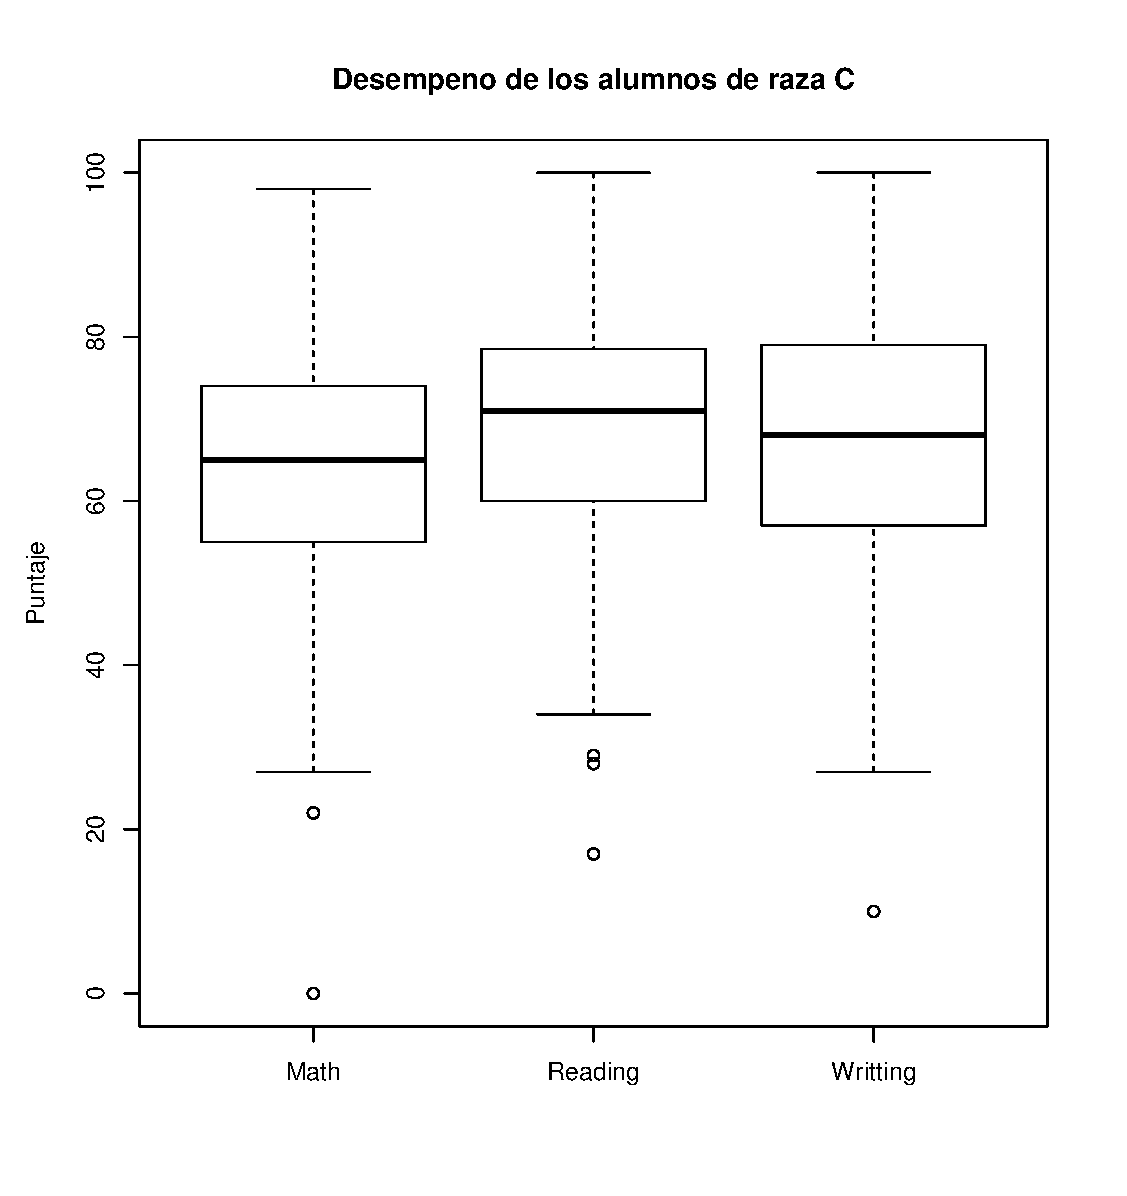
\includegraphics[scale = 0.6]{Output/Plots/DesempenoAlumnosRazaC.eps}
    \caption{Desempe\~no alumnos de raza C}
    \label{fig:minipage1}
\end{figure}

En conjunto, salvo algunas excepciones, este grupo logr\'o notas por encima de 50 pts, lo cual puede indicar ciertos
patrones de estudio o elementos que puedan haber ayudado a lograr estas notas.

Por otro lado podemos notar la correlaci\'on que existe entre los puntajes de las materias

\begin{figure}[H]
    \centering
    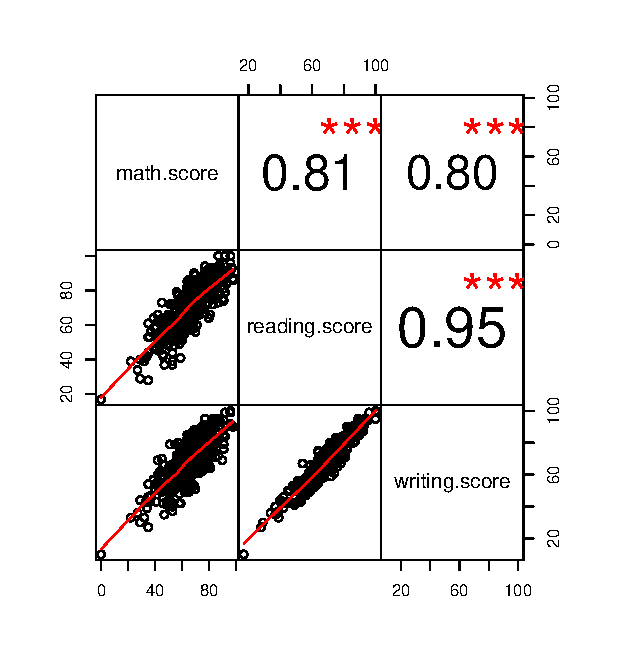
\includegraphics[scale = 0.9]{Output/Plots/5Correlation.eps}
    \caption{Correlaci\'on entre puntajes}
\end{figure}

De la figura 3 podemos ver la alta correlaci\'on que existe entre las notas, en especial entre Writting y Reading. En general
un alumno de este grupo que haya salido bien en una materia es muy probable que suceda lo mismo en las dem\'as. Lo cual
puede significar que aquellos alumnos que salieron mal en alguna no es por una dificultad propia de la materia sino por 
condiciones propias del alumno.

Podemos utilizar la distancia de Mahalanobis para verificar cu\'antos alumnos est\'an relaivamente alejados del centroide
representado por los datos de las notas.


\begin{figure}[H]
    \centering
    \includegraphics[scale = 0.9]{Output/Plots/DistanciaMahalanobis.eps}
    \caption{Distancia de Mahalanobis}
\end{figure}

Viendo la figura 4 podemos ver que son pocos los alumnos muy alejados del centroide definido por los puntajes obtenidos,
significando que los casos en los que los alumnos, para bien o para mal, se alejan de la media son at\'ipicos.

Para determinar los posibles factores que contribuyeron a que algunos alumnos hayan podido salir mal, analizaremos seg\'un
las caracteristicas dadas por los alumnos.

\begin{figure}[H]
    \centering
    \includegraphics[scale = 0.9]{Output/Plots/ProcentajeGenero.eps}
    \caption{Distancia de Mahalanobis}
\end{figure}
\begin{figure}[ht]
    \centering
    \begin{minipage}[b]{0.45\linewidth}
        \includegraphics[width=8cm]{Output/Plots/DesempenoMaculino.eps}
        \caption{Desempeno genero masculinos}
        \label{fig:minipage1}
    \end{minipage}
    \hspace{0.2cm}
    \begin{minipage}[b]{0.45\linewidth}
        \includegraphics[width=8cm]{Output/Plots/DesempenoFemenino.eps}
        \caption{Desempeno genero Femenino}
        \label{fig:minipage2}
    \end{minipage}
\end{figure}


\end{document}